\section*{KNN}

We want to approximate $f: \mathcal{X} \to \mathcal{Y}$, $\mathcal{X} \in \mathbb{R}^p$, $\mathcal{Y}=\{1,...,L\}$ \\

We note:

$x=(x_1,...,x_p)^T \in \mathcal{X}$ a sample

The distance between 2 samples: $d: \mathbb{R}^p \times \mathbb{R}^p \to \mathbb{R}$

$\mathcal{D}_n=\{(x_i,y_i),i=1,...,n\}$ the training set with $n$ samples and labels. \\

For each new sample $x \in \mathbb{R}^p$, we determine the set of k nearest neighbors among all the train set. \\

\textit{Note}: a sample is an observation, that is $x^T=(x_i^{(1)},...,x_i^{(p)})$. We thus compute the distances between \textbf{vectors} of dimension $p$.

The most basic distance metric is the Euclidean norm: $d(u,v)=||u-v||^2=\Sigma_{i=1}^p(u_i-v_i)^2$ \\

The algorithm consists in building a distance matrix with the test sample in columns (power $(t)$) and the train sample in rows (power $(T)$) as shown below:

\begin{center}
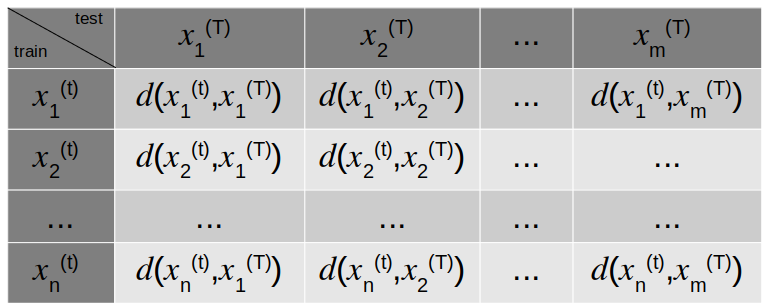
\includegraphics[scale=0.3]{KNN_matrix.png}
\end{center}

\textit{Note}: in this matrix, the training sample is of size $n$ and the test sample is of size $m$. \\

We then sort the matrix column-wise in ascending order in order to find train data points with smallest distance to the test data point. \\

For each test data point, we keep the $k$ smallest distances (i.e. the $k$ first rows of the sorted matrix) and we look at their labels. The Python function \textit{argsort()} allows us to keep indices when sorting. We define the rank of a neighbor as:  \\

$$r_k(x)=i^* \text{ if and only if:}$$ $$d(x_{i^*},x)=\underset{1 \le i \le n,~ \\
i \neq r_{1},...,r_{k-1}}{\operatorname{min}}d(x_i,x)$$ \\

The most basic rule is to take the most frequent label among the $k$ neighbors. In the below schema we consider $k=5$ and $k=11$ with three classes ($L=3$) that are drawn respectively in black ($y=1$), grey ($y=2$) and white ($y=3$).

$$\widehat{f}_k(x)=\underset{y \in \mathcal{Y}}{\operatorname{argmax}}(\Sigma_{j=1}^k \mathbbmss{1}\{y_{r_j}=y\})$$

\begin{figure}[h!]
\begin{center}
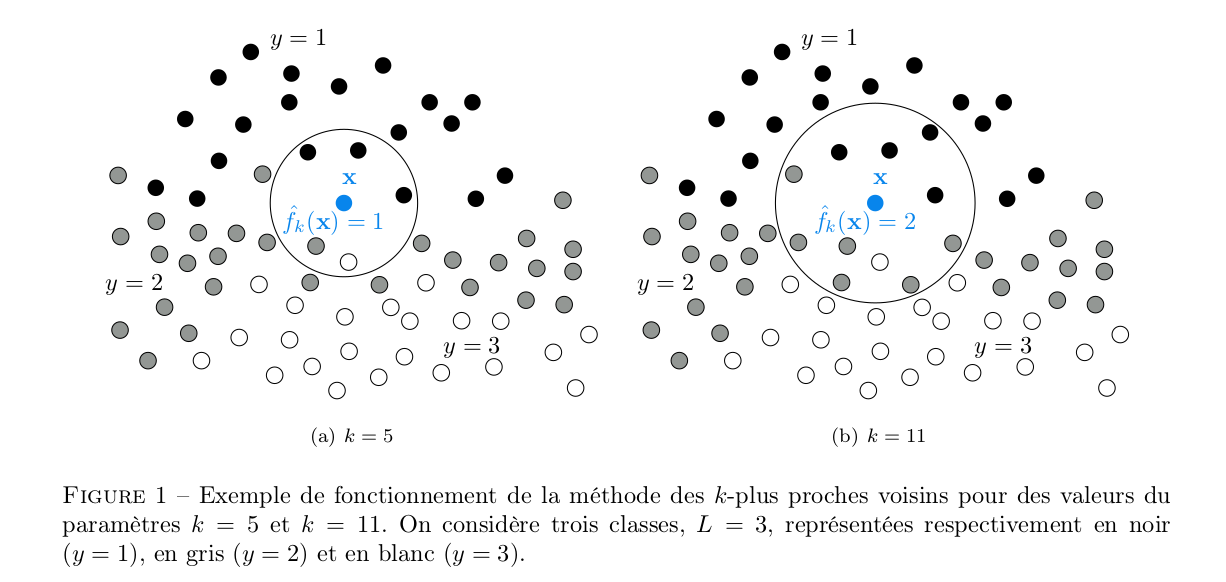
\includegraphics[scale=0.4]{KNN_pic.png}
\caption{Example of KNN prediction}
\end{center}
\end{figure}

\textit{Note}: the \textit{fit()} function of the \textit{KNNClassifier} is just an affectation of the training data to the object; the distance computation is done in the \textit{predict()}. \\

The biggest advantages of the KNN algorithm are:

- It's a simple and intuitive algorithm that can be easily explained and understood.

- Its parameter can be easily optimize e.g. using cross validation.

The biggest drawbacks are:

- The prediction can be greedy to compute because we need to compute all distances between test and train data.

- It has a high variance: the prediction can be strongly different if the data are slightly different. \\

\textbf{Alternative}

$$\widehat{f}_k(x)=\underset{y \in \mathcal{Y}}{\operatorname{argmax}}(\Sigma_{j=1}^k \omega_j \mathbbmss{1}\{y_{r_j}=y\})$$

$$\text{where:}$$

$$\omega_j = e^{-d_j^2/h}$$

This alternative doesn't change the knn selection, it only changes the class attribution in the neighborhood. It gives more weights to very small distances. The higher $h$, the higher we favor small distances ($exp$ function becomes steeper).

\lstset{language=Python}
\lstset{frame=lines}
\lstset{caption={KNN algorithm}}
\lstset{label={lst:code_direct}}
\lstset{basicstyle=\footnotesize}
\begin{lstlisting}

class KNNClassifier(BaseEstimator, ClassifierMixin):
    """ Homemade kNN classifier class """
    def __init__(self, n_neighbors=1):
        self.n_neighbors = n_neighbors
    
    # the training step only consists in storing training data
    def fit(self, X, y): 
        self.X = X
        self.Y = y
        return self
    
    def predict(self, X):
        n = len(self.X) # size of train set
        m = len(X) # size of test set
        dist_mat = []
        for i in range(n): # we loop on every element of the train set
            dist_vect = []
            for j in range(m): # we loop on every element of the test set
                dist_vect.append(euclidean_distance(self.X[i], X[j]))
            dist_mat.append(dist_vect) 
	  # len(dist_vect) = m (nb of features; all the distances for one observation)
            
        dist_mat = np.asarray(dist_mat) 
        # dist_mat.shape = (n,m); T_test in column, X_train in row
        
        # dist_mat = metrics.pairwise.pairwise_distances(
				X, Y=self.X, metric='euclidean', n_jobs=1
				)
            
        idx_sort = np.argsort(dist_mat, kind='mergesort', axis=0)  
        # idx_sort.shape = (n,m); dist_mat sort column-wise
        # mergesort is a stable way to handle equal numbers: 
        # if equal, the order of indices in the output is the same as in the input
        
        idx_sort_knn = idx_sort[:self.n_neighbors,:] # resize with the number of knn
        return getBestClassFromCount(idx_sort_knn, self.Y) 

\end{lstlisting}

\vspace{5mm}